%% Преамбула TeX-файла

% 1. Стиль и язык
\documentclass[utf8x, 14pt]{G7-32} % Стиль (по умолчанию будет 14pt)

% Остальные стандартные настройки убраны в preamble.inc.tex.
\sloppy

% Настройки стиля ГОСТ 7-32

% Добавляем гипертекстовое оглавление в PDF
\usepackage[
bookmarks=true, colorlinks=true, unicode=true,
urlcolor=black,linkcolor=black, anchorcolor=black,
citecolor=black, menucolor=black, filecolor=black, urlcolor=blue,
]{hyperref}
\AfterHyperrefFix

\usepackage{microtype}% пакет для микротипографии, под pdflatex хорошо улучшает читаемость

% Тире могут быть невидимы в Adobe Reader
\ifInvisibleDashes
\MakeDashesBold
\fi

\usepackage{graphicx}   % Пакет для включения рисунков
\usepackage{tikz}
\graphicspath{ {./images/} }

\geometry{right=20mm}
\geometry{left=30mm}
\geometry{bottom=20mm}
\geometry{ignorefoot}


\setlength{\parskip}{1ex} % разрыв между абзацами

% Упрощение написания ссылки
\newcommand\case[1]{По Случаю #1 из Теоремы 2.6 из \cite{hse:Teoria_Gener}}





% Стиль титульного листа и заголовки
% Титульная страница, по умолчанию ГОСТ 7.32-2001,  
 
\NirOrgLongName{Правительство Российской Федерации\par
Федеральное государственное автономное образовательное\\
учреждение высшего образования\\
"Национальный исследовательский университет\\
"Высшая школа экономики"\\
Московский институт электроники и математики им. А.Н. Тихонова\\
Департамент прикладной математики
} 


\NirReportName{Методические материалы}
\NirAbout{По дисциплине \par "Теория псевдослучайных генераторов"} 


\Nir{Разбор практических задач с теоретическим обоснованием}

\NirSubject{Типовые задачи контрольных работ}                                
\NirCode{}

\NirManager{Преподаватель дисциплины}{М.И. Рожков }
\NirIsp{Руководитель создания документа}{А.Ю. Нестеренко}

\NirYear{2021}
\NirTown{Москва}



\begin{document}

\frontmatter % выключает нумерацию; здесь начинаются НЕнумерованные главы: введение, глоссарий, сокращения.

\maketitle % создает титульную страницу


\begin{executors}
\personalSignature{Выполнил студент}{Щеглова П.Н.}
\end{executors}

\tableofcontents % создает содержание документа
 

\Introduction

Целью работы является демонстрация навыков подготовки электронных документов в системе компьютерной верстки документов latex. Выполнены требования к подготавливаемому документу:

\begin{itemize}
\item титульный лист по ГОСТ 7.32-2001;
\item общий объем документа не менее 18 страниц;
\item наличие разделов документа, включая ненумерованные (введение, обозначения и т.п.);
\item наличие формул (строчные и выключенные);
\item наличие ссылок (по документу и внешних);
\item наличие таблиц, изображений и т.п.;
\item наличие списка литературы и ссылок на него по тексту документа;
\item определение собственных команд, упрощающих процесс набора документа;
\item отсутствие орфографических ошибок, наличие смысла в подготовленном документе,
обоснование, для чего документ подготовлен;
\item краткая информация о сборке документа и используемых шрифтах, размерах (шрифтов, полей и т.п.);
\item информация о том, какие стилевые пакеты применяли и для какой цели.
\end{itemize}

Содержательно документ подготовлен для демонстрации студентам, проходящим курс теории псевдослучайных генераторов, хода решения типовых задач из контрольноых работ, для некоторых типов задач приведено решение для всех вариантов входных параметров. Первыми разбираются общие задачи для двух контрольных, затем уникальные для первой контрольной задачи и для второй. Теоретические обоснования даны в виде ссылок на соответствующие утверждения из источников и частично продублированы в виде утверждений. 
 % создает раздел Введение


\mainmatter % это включает нумерацию глав и секций в документе ниже

\chapter{Шифрование с сохранением формата}

\section{Описание концепции}
Format-preserving encryption (FPE) --- это семейство перестановок на произвольном множестве $\mathcal{S}$, индексируемое ключом $K$ \cite{ruscrypto}
$$FPE_K: \mathcal{S} \to \mathcal{S}.$$
 Примеры отображений: шифрование 16--значного номера банковской карты 16--значным числом; шифрование одного английского слова другим английским словом. Блочный шифр --- частный случай FPE--схемы, для которой  $\mathcal{S} = \{0,1\}^n$, где $n$ --- длина блока.


Истинно случайная перестановка является идеальным шифром FPE, однако для больших множеств невозможно предварительно сгенерировать и запомнить такую перестановку. Таким образом, проблема FPE состоит в том, чтобы сгенерировать псевдослучайную перестановку из секретного ключа так, чтобы время вычисления для одного значения было небольшим (в идеале постоянным, но, что наиболее важно, меньшим, чем $O(n)$, где $n$ - размер входных данных).


Алгоритм FPE можно реализовать с использованием сети Фейстеля. Например, стандарты FF1 и FF3-1 \cite{FF13-1} берут за основу алгоритма сеть Фейстеля, а в качестве раундовой функции шифрования части входных данных $F$ стандартизированный блочный шифр с блоками длины 128 бит (AES).


\section{Действующие стандарты} % Добавить ссылки на стандарты
Существует множество реализованных алгоритмов типа FPE, к действующим можно отнести разработанные в США FF1 и FF3-1 \cite{FF13-1}, а также южно-корейские FEA-1 и FEA-2 \cite{FEA}.
Алгоритм FEA, представленный институтом исследований национальной безопасности (NSR), также основан на сети Фейстеля, аналогично стандартам NIST, FF1 и FF3-1. 


Разница между FEA-1 и FEA-2 состоит в том, что FEA-1 имеет размер настройки (параметра, подающегося на вход раундовой функции $F$) $128-n$ бит (где $n$ - размер входной последовательности), каждый с 12, 14 и 16 раундами при длине двоичного ключа 128, 192 и 256, соответственно. FEA-2 имеет фиксированный размер настройки в 128 бит с 18, 21 и 24 раундами при длинах ключей 128, 192 и 256, соответственно.

\subsection{FEA-1}
Опишем подробнее стандарт, который анализируется в данной работе, а именно FEA-1:

На вход алгоритму подаются последовательности чисел из конечного множества, мощностью от $2^8$ до $2^{128}$, размер двоичного ключа $K$ может составлять 128, 192 или 256 бит. Алгоритм представляет собой последовательное применение итераций сети Фейстеля, ее общая схема представлена в левой части рисунка \ref{fig:fea_structure}. Входная последовательность $X$ на каждом раунде делится на две равные части $X_a$ и $ X_b$, $X_b$ передается на вход $F$-функции, общая схема которой обозначена в правой части рисунка \ref{fig:fea_structure}: $T_a$ и $T_b$ - левая и правая половины настройки, принцип формирования которой будет описан далее, $RK_a$ и $RK_b$ - левая и правая половины раундового ключа, $S$ - блок подстановки (в данной схеме применяются идентичные $S$-блоки), $\mathcal{M}$ - блок умножения на заданную матрицу.

\begin{figure}[h!]
	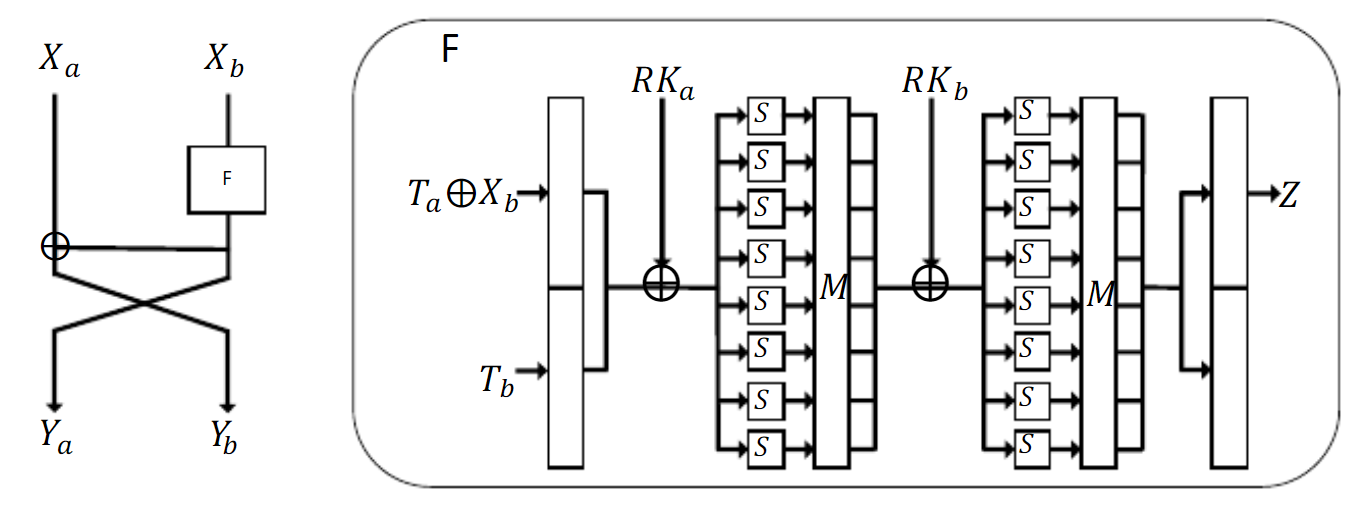
\includegraphics[width = \textwidth]{FEA-1 structure.png}
	\caption{Структура итерации FEA, на основе сети Фейстеля}
	\label{fig:fea_structure}
\end{figure}

Выбор настройки для каждого раунда происходит по следующему алгоритму: настройка $T$ (битовый вектор длины $128-n$) делится на две под-настройки $T_L = T_{ [ 0:64-n_2-1 ] }$ и $T_R=T_{ [ 64-n_2:128-n-1 ] }$ длины $64-n_2$ и $64-n_1$, соответственно. Полагаем $T_a^i=0$ для каждой итерации и $T_b^i$ для $i$-ой итерации, как:

$$ T_b^i =
\begin{cases}
T_L & \dfrac{i}{2} \in N \\
T_R & \dfrac{i+1}{2} \in N
\end{cases} $$

\chapter{Линейный метод}
\section{Схема и обозначения}
Сначала опишем общую схему алгоритма и обозначения для применения линейного метода криптоанализа.

Известно $T$ пар открытых текстов и соответствующих шифртекстов $(a^{(i)}, c^{(i)}), i\in\overline{1,T}$, каждый из которых состоит из $N$ бит: $a_1^{(i)}, ..., a_N^{(i)}$ и $c_1^{(i)}, ..., c_N^{(i)}$. Пусть схема шифропреобразования с ключом $K$ разбита на две последовательные части $F_{K_1}$ и $F_{K_2}$, как показано на рисунке \ref{fig:linan}. 
\begin{figure}[h!]
	\centering
	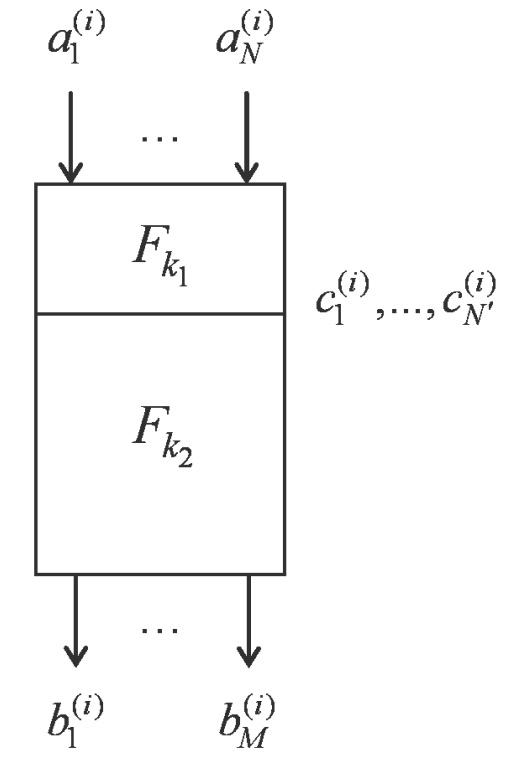
\includegraphics[scale=0.25]{linan.png}
	\caption{Схема разбиения алгоритма на два блока для проведения линейного криптографического анализа}
	\label{fig:linan}
\end{figure}
В первой из них используется часть исходного ключа $K_1$, во второй, соответсвенно, $K_2$ (при этом $K_1$ может частично совпадать с $K_2$). $F_{K_1^{'}}(a^{(i)}) = b^{(i)} = b_1^{(i)}, ..., b_N^{(i)}$ -- промежуточный шифртекст, зашифрованный на некотором ключе $K_1^{'}$. $\alpha = \alpha_1, ..., \alpha_N; \beta = \beta_1, ..., \beta_N$ -- битовые маски, которые мы будем накладывать на промежуточный и итоговый шифртексты, соответственно. Наложение маски подразумевает cкалярное произведение двух векторов: $(\alpha, b^{(i)}) = (\alpha_1 \cdot b_1^{(i)}) \oplus ... \oplus (\alpha_N \cdot b_N^{(i)})$.

Для отбраковывания ложных ключей линейный метод предполагает проверку выполнения некоторого соотношения с нужной вероятностью. Для двух масок $\alpha \in \mathbb{F}_2^n$ и $\beta \in \mathbb{F}_2^m$ и функции $F :\mathbb{F}_2^n \to \mathbb{F}_2^m$ определим следующую величину:

$$ \delta_{\alpha, \beta}^{F} = 2\cdot P\left( (\alpha, x) = (\beta, F(x)), x\in \mathbb{F}_2^n\right) - 1 = \dfrac{1}{2^n} \sum_{x\in \mathbb{F}_2^n} (-1)^{(\alpha, x) + (\beta, F(x))}$$

Для равномерно распределенной функции $F :\mathbb{F}_2^n \to \mathbb{F}_2^m$ справедлива следующая теорема:
\section{Теорема (\cite{Daemen})}\label{theorem}

 Пусть определена $\delta_{\alpha, \beta}^{F}$ для равномерно распределенной функции $F: \mathbb{F}_2^n \to \mathbb{F}_2^n$. Тогда случайная величина $\xi = 2^{n-1}(\delta_{\alpha, \beta}^{F}+1)$ имеет биномиальное распределение с математическим ожиданием $M\xi = 2^{n-1}$ и дисперсией $D\xi = 2^{n-2}$. В частности, при $n\to\infty$ распределение $2^{n/2}\delta_{\alpha, \beta}^{F}$ сходится к стандартному нормальному распределению $\mathcal{N}(0,1)$.


\section{Алгоритм метода}
Перейдем к описанию алгоритма. $\alpha$ и $\beta$ заданы, вычислено теоритическое значение $\delta_{\alpha, \beta}^F$, вычислен доверительный интервал. Для каждого $K_1^{'}$:

\begin{enumerate}
    \item Полагаем $\overline{P} = 0$;
    \item Для каждого $a^{(i)}, i\in\overline{1,T}$, вычисляем $b^{(i)} = F_{K_1^{'}}(a^{(i)})$; 
    \item Проверяем выполнено ли равентсво $(\alpha, b^{(i)}) = (\beta, c^{(i)})$. 
    \item Если равенство выполнилось, полагаем $\overline{P} = \overline{P} + 1$
    \item После перебора материала полагаем $\overline{P} = \dfrac{\overline{P}}{T}$;
    \item Если $\overline{P} \backsimeq P$, считаем, что часть ключа $K_1 = K'_1$, при необходимости продолжаем работу с $F_{K_2}$ по той же схеме.
    \item Иначе, отбрасываем ключ $K'_1$ как ложный, выбираем новый и повторяем все итерации.
\end{enumerate}

Чем больше при этом $T$ и $|\delta_{\alpha, \beta}^F|$, тем большая доля значений $K_1^{'}$ будет отбракована на каждой итерации, вплоть до однозначного определения $K_1^{'}$.

Для того, чтобы применить вычисляемую оценку для отбраковывания ложных ключей, необходим различитель, который на основе теоритической $\delta$ определяет, выполнилось ли соотношение с нужной вероятностью. Чтобы построить различитель, воспользуемся результатами, полученными в \cite{main_paper}.


\section{Теоритические выкладки из \cite{main_paper}}
Пусть $F: \mathbb{F}_2^n \to \mathbb{F}_2^n$ - наша раундовая функция, $n$ - размер блока. Различитель строится на основе линейных соотношений с большой $\delta$. Линейное соотношение для $F$ определяется двумя масками $(L^{'}, L^{''}) \in \mathbb{F}_2^n \oplus \mathbb{F}_2^n$, и их $\delta$ равна:
$$ \delta_{L^{'}, L^{''}}^{F} = 2\cdot P\left(L^{'} \& F(x) = L^{''} \& x\right)-1 ,$$
где вероятность считается от равномерно распределенного открытого текста  $x\in \mathbb{F}_2^n$, а \& означает побитовое наложение маски на текст. Если $L^{'} \neq 0$, то математическое ожидание $\delta$ равновероятно распределенной функции равно нулю, а стандартное отклонение $\sigma = 2^{-n/2}$. Следовательно, если $\hat{\delta}$ значительно превосходит $2^{-n/2}$, то различителем можно считать вычисление $\hat{\delta}$ для возможных пар масок и сравнение получившего значения с некоторым заданным пороговым значением.

Основное наблюдение \cite{main_paper}, которое можно эксплуатировать в атаках на FPE шифры, состоит в том, что шифр оказывается нестойким, если настройка (её часть) считается частью входных данных.


Рассмотрим два раунда FEA-1 (рисунок \ref{fig:trial}), настройка $T_L$ - произвольная постоянная, а $T_R$ считается переменной входа. Если это не так, то для проведения атаки $T_R$ должна быть известной. Идея атаки состоит в том, что $\delta$  линейного соотношения раундовой функции $F_r$ превышает $ 2^{-n/2}$ с достаточно большой вероятностью, что важно, когда настройка включается во входные данные, потому что область определения функции, которая отображает настройку и открытый текст в шифртекст, велика. Математическое ожидание $\delta$ линейных соотношений над случайной функцией с тем же размером входа (включая $T_R$ размера $64-n_1$), что и в FEA-1, равно нулю, а стандартное отклонение $2^{-32-n_1/2}$. 

\begin{figure}[h!]
	\centering
	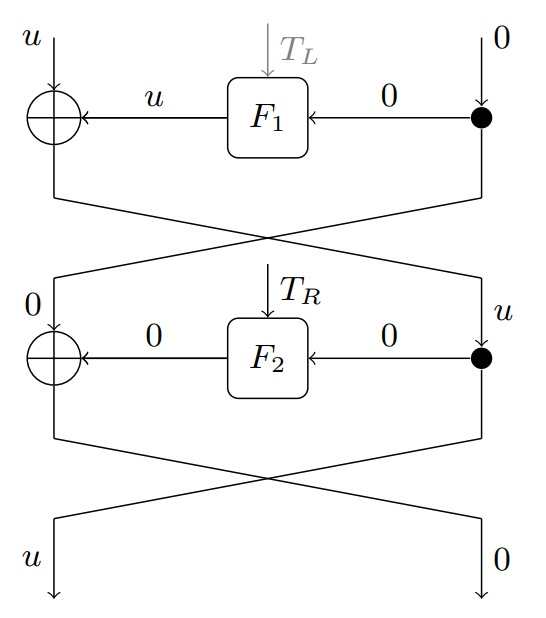
\includegraphics[scale=0.5]{trial.png}
	\caption{Две итерации FEA-1}
	\label{fig:trial}
\end{figure}


\subsection{Применение}

Пусть $r\geq 2$ - четное целое число. $\delta$ для $r$ раундов равна $\delta=\prod_{i=1}^{r/2} \delta_i$, где $\delta_i \thicksim \mathcal{N}(0,1/\sqrt{N})$ по теореме \ref{theorem}, $N$ --- мощность множества текстов. Переменнные $\delta_i$ будем считать независимыми, что следует из предположения о независимости раундовых функций $F_1, F_3, ..., F_{r-1}$.

Эвристически вычислимо, что для FEA-1
\begin{equation}
\label{eqn:keyeq}
1/\mathbb{E}(\delta^2)=\sqrt{N}^{r/2},\end{equation} 
где $\mathbb{E}(\delta^2)$ - средне-квадратичная $\delta$ для равномерно распределенного случайного ключа.


\chapter{Эксперимент}
Теперь проведем эксперимент: возьмем все возможные тексты размера 8 бит, сгенерируем произвольный ключ длины 128 бит, зафиксируем произвольной константой первую часть настройки и будем проведить шифрование алгоритмом FEA-1 всего в два раунда. Зафиксируем число $\alpha \in \overline{1,15}$ и зададим две маски: $\alpha|0$ и $0|\alpha$. Для каждой второй части настройки сгенерированной произвольно 1000 раз, для каждого открытого текста из множества производим зашифрование, с помощью полученного шифртекста получаем квадрат оценки $\hat{\delta}$ для первой маски (и на входе, и на выходе маска берется одна и та же) и квадрат оценки для второй маски, усредняем оценки по всем настройкам. 

$1/\mathbb{E}(\delta^2)=\sqrt{N}^{r/2} = (2^4)^{2/2} = 2^4, \mathbb{E}(\delta^2) = 0.0625$

Реализацию эксперимента можно найти по \href{https://github.com/jerrydie/course_work}{ссылке}. Для каждого $\alpha$ результаты следующие:

\begin{center}
\begin{tabular}{ |p{0.1\textwidth}| p{0.2\textwidth}| p{0.2\textwidth}| }
\hline
 $\alpha$ & $\delta(0|\alpha )$ & $\delta(\alpha|0)$ \\
 \hline
1 & 0.0625 & 0.0863125 \\
2 & 0.0625 & 0.0571562 \\
3 & 0.765625 & 0.330266 \\
4 & 0.25 & 0.0562344 \\
5 & 0.5625 & 0.334469 \\
6 & 0.765625 & 0.322062 \\
7 & 1 & 0.6155 \\
8 & 0.015625 & 0.0683437 \\
9 & 0.5625 & 0.322297 \\
10 & 0.25 & 0.328 \\
\hline
\end{tabular}
\end{center}

\section{Выводы}
В результате работы был разобран линейный метод криптографического анализа шифров, сохраняющих формат. Для проверки теоритических изысканий была создана программа для проведения эксперимента по нахождению линейного соотношения между открытыми текстами, к которым применятся алгоритм шифрования FEA-1, и соответствующими шифртекстами. Результаты эксперимента коррелируют с теорией, однако требуется дальнейшее изучение с целью обобщения теоритических результатов и описания способов атак на FPE шифры.
% \cite{hse:Teoria_Gener} любой характеристический многочлен ЛРП кратен минимальному многочлену. Тогда достаточно проверить делители характеристической функции.





\backmatter %% Здесь заканчивается нумерованная часть документа и начинаются ссылки

% % Список литературы при помощи BibTeX
% Юзать так:
%
% pdflatex main
% bibtex main
% pdflatex main

\bibliographystyle{ugost2008}
\bibliography{main}

%%% Local Variables: 
%%% mode: latex
%%% TeX-master: "main"
%%% End: 



%\appendix   % Тут идут приложения

%\include{90-appendix1}

%\include{91-appendix2}

\end{document}

%%% Local Variables:
%%% mode: latex
%%% TeX-master: t
%%% End:
